\clearpage

\section{Optical Attenuator}

\begin{tcolorbox}	
\begin{tabular}{p{2.75cm} p{0.2cm} p{10.5cm}} 	
\textbf{Header File}   &:& optical\_attenuator\_20180304.h \\
\textbf{Source File}   &:& optical\_attenuator\_20180304.cpp \\
\textbf{Version}       &:& 20180304 (\textbf{Student Name}: Mariana Ramos)
\end{tabular}
\end{tcolorbox}


This block of code simulates the attenuation in optical fibre, which is basically the reduction of intensity of the light beam with respect with the distance of the communication channel. 





\subsection*{Functional description}

\begin{figure}[h!]
	\centering
	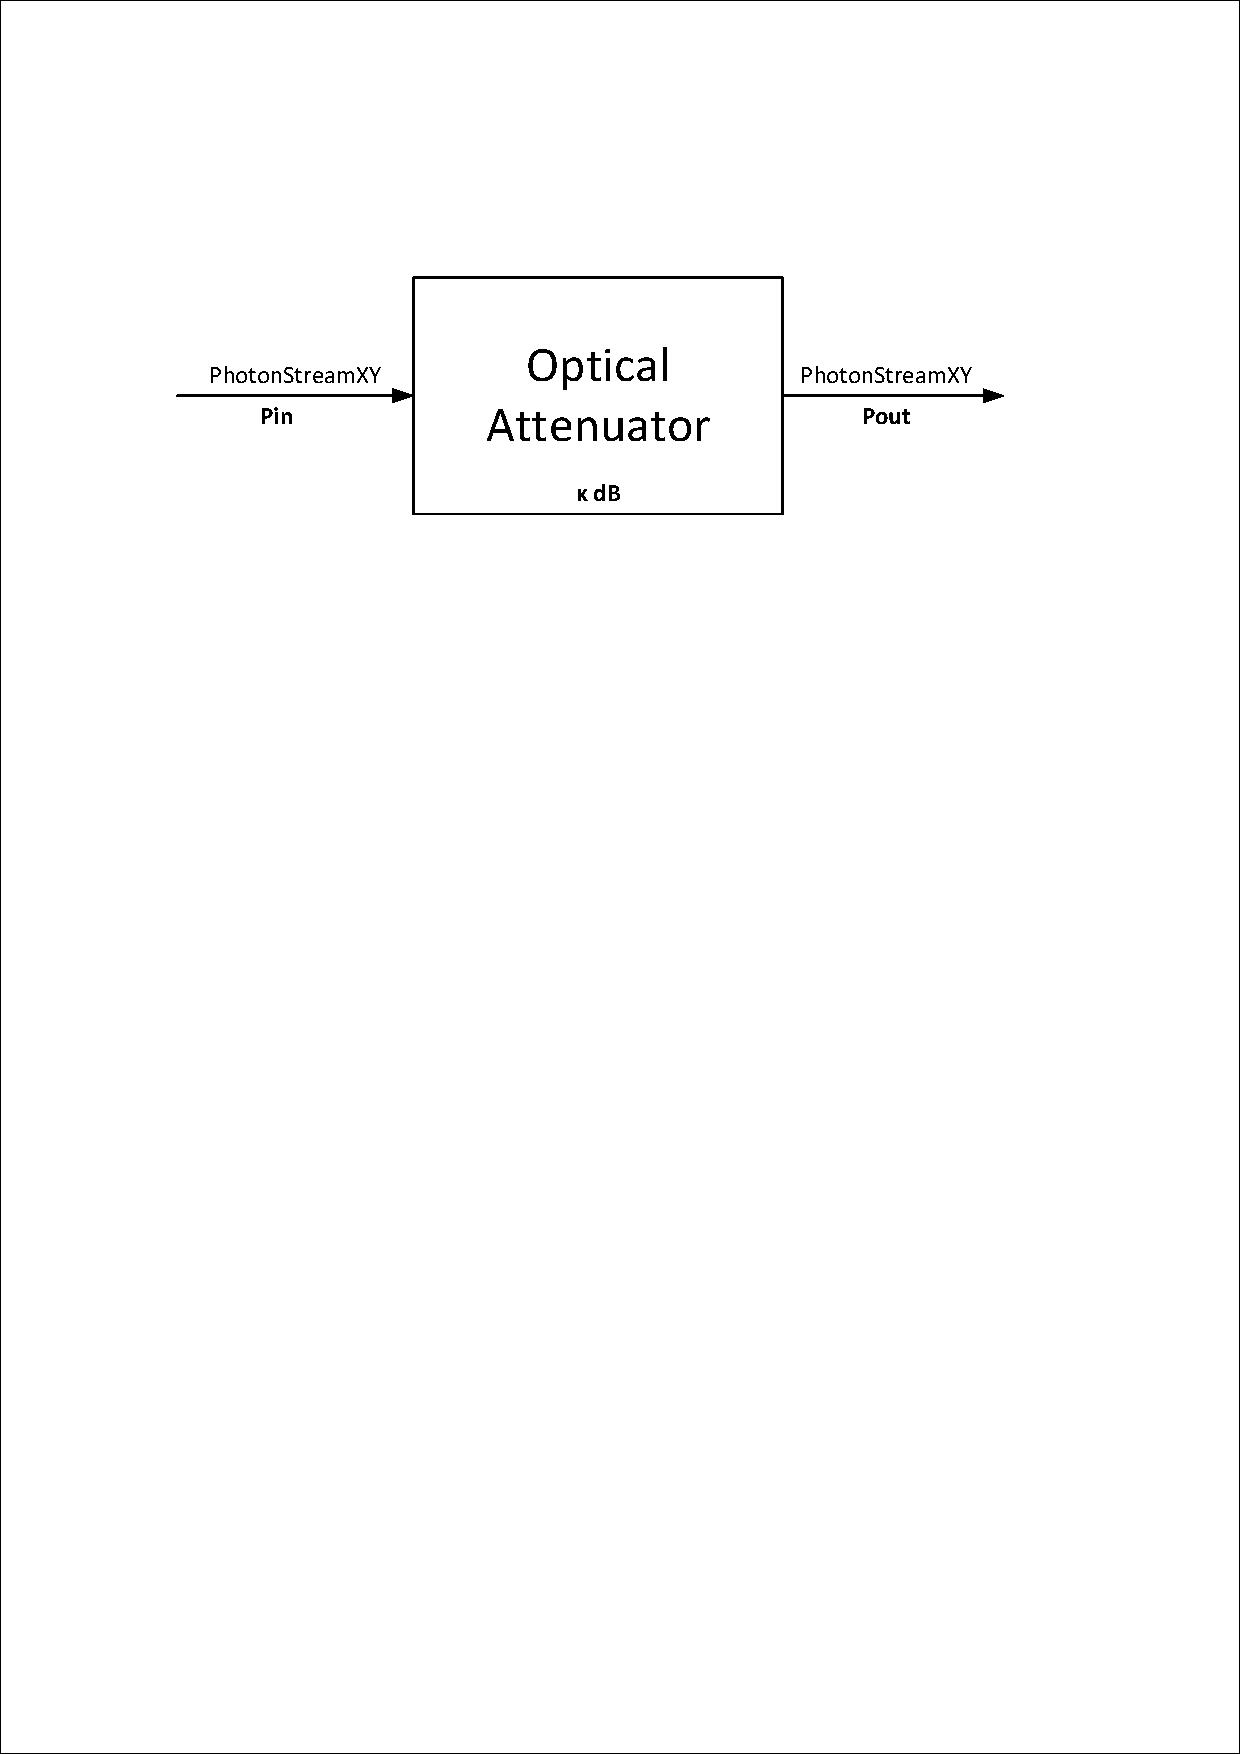
\includegraphics[clip, trim=3cm 20cm 4cm 4cm, width=0.60\textwidth]{../lib/optical_attenuator/figures/diagram.pdf}
	\caption{Optical Attenuator diagram}\label{fig:diagram}
\end{figure}

As one can see in figure \ref{fig:diagram} this block accepts an optical photon stream XY signal and outputs the same type of signal.

The optical attenuator intends to simulate the attenuation in optical fiber which means a decrease of intensity in the input beam due transmission losses in the quantum channel with respect to distance travelled by the single photon over the optical fibre communication channel.

This attenuation can be represented by a value $\kappa_{dB}$ in dB, which is one of the input parameters of this block. By definition, the attenuation can be calculated using the following equation:

\begin{eqnarray}
\label{eq:attenuation}
% \nonumber % Remove numbering (before each equation)
  \kappa_{dB}   &=& -10 \log_{10}\left(\frac{P_{out}}{P_{in}}\right) \\
  \nonumber
                &=& -10 \log_{10}\left(\frac{2|A_{out}|^2}{2|A_{in}|^2}\right) \\
  \nonumber
                &=& -10 \log_{10} \textit{kappa}^2 \\
  \nonumber
                &=& -20 \log_{10} \textit{kappa}
\end{eqnarray}

In equation \ref{eq:attenuation}:

\begin{equation*}
  A_{in} = \left[
  \begin{array}{c}
    Ax_{in} \\
    Ay_{in}
  \end{array} \right]
\end{equation*}

and, 

\begin{equation*}
  A_{out} = \left[
  \begin{array}{c}
    Ax_{out} \\
    Ay_{out}
  \end{array} \right],
\end{equation*}

which are the input photon stream and the output photon stream, respectively, represented by an array of two complex numbers.

Afterwards,

\begin{equation}\label{eq:relation}
  A_{out} = \textit{kappa} A_{in},
\end{equation}

and \textit{kappa} can be calculated using the input parameter $\kappa_{dB}$ by the following equation:

\begin{equation}\label{eq:kappa}
  \textit{kappa} = 10 ^{-\frac{\kappa_{dB}}{20}}.
\end{equation}


\subsection*{Input parameters}

 In the following table (table~\ref{table:sopmodulator_in_par}) the input parameters and corresponding functions of the optical attenuator block are summarized.

\begin{table}[h]
	\centering
	\begin{tabular}{|c|c|c|c|cccc}
		\cline{1-4}
		\textbf{Parameter} & \textbf{Type} & \textbf{Values} &   \textbf{Default}& \\ \cline{1-4}
		k & double & any & 0.0 \\ \cline{1-4}
	\end{tabular}
	\caption{List of input parameters of the block Optical Modulator}
	\label{table:sopmodulator_in_par}
\end{table}


\subsection*{Methods}


	OpticalAttenuator(vector <Signal*> \&inputSignals, vector <Signal*> \&outputSignals)(\textbf{constructor})
\bigbreak
	void initialize(void)
\bigbreak
	bool runBlock(void)
\bigbreak
	void setAttenuationCoef(double coef)
\bigbreak
	double getAttenuationCoef()
\bigbreak



\subsection*{Input Signals}

\subparagraph*{Number:} 1

\subparagraph*{Type:} PhotonStreamXY

\subsection*{Output Signals}

\subparagraph*{Number:} 1

\subparagraph*{Type:} PhotonStreamXY

\subsection*{Example}

\subsection*{Sugestions for future improvement}
